\subsection{When monopoly eliminates AI-dominated growth}
\label{subsec:rewrite-monopoly-growth-reversal}

I now ask whether monopoly can eliminate AI-dominated growth even while
research makes AI more efficient. This is the opposite outcome to the
preceding exercise: research gains fail to compensate for restricted AI use.
Following Corollary~\ref{cor:rewrite-monopoly-bottleneck}, I choose
$\sigma=1.5$ and
$\mathcal B^{\mathrm{mc}}(1.5)<B_0<\overline B<\mathcal B(1.5)$.
Initial efficiency is high enough for AI-dominated growth under
competition, but even the upper bound is insufficient under monopoly.
The unexpected grant covers existing technology and future improvements,
as in Section~\ref{subsec:rewrite-competitive-transition}. RSI is
available throughout; the grant changes pricing and research incentives.

Table~\ref{tab:rewrite-monopoly-growth-reversal} reports the new design.
I retain the other parameters in Table~\ref{tab:rewrite-rsi-parameters}
and compare continued competition with monopoly under $\chi=7.5$ and
$\chi=1.5$, all from the same initial stocks. Before granting monopoly
rights, I let the competitive economy approach its AI-dominated
growth path. I select the first whole year when output-per-worker growth,
wage growth, and the interest rate are each within 0.1 percentage point
of their long-run limits, and reset the date to zero. I inherit $A_0$,
$N_0$, and $K_0$ jointly from that date, keeping $B_0$ and both values of
$\chi$ unchanged. This is a near-long-run competitive allocation, not
an exact steady state: $K/(AL)$ continues to grow. Just before the grant,
output per worker grows at $5.8\%$, wages at $4.2\%$, and the interest
rate is $9.8\%$. The capital--output ratio is 2.23.

\begin{table}[H]
 \centering
 \caption{Parameters and initial stocks for the growth-reversal experiment}
 \label{tab:rewrite-monopoly-growth-reversal}
 \small\setstretch{1.0}
 \begin{tabular}{ccl}
 \toprule
 Object & Value & Choice\\
 \midrule
 $\sigma$ & 1.5 & Substitution\\
 $\chi$ & 7.5; 1.5 & Same illustrative research productivities\\
 $\overline B$ & 1,113.5 & $0.90\mathcal B(1.5)$\\
 $B_0$ & 1,002.2 & $0.90\overline B$\\
 $A_0,N_0$ & 6.6859; 1.7683 & Inherited from competitive prehistory\\
 $K_0$ & $7.2907\times10^9$ & Inherited from the same date\\
 $K_0/Y_{0^-}$ & 2.23 & Competitive ratio before the grant\\
 \bottomrule
 \end{tabular}
 \par\vspace{4pt}
 \parbox{0.95\textwidth}{\footnotesize\emph{Notes:}
 $\mathcal B^{\mathrm{mc}}(1.5)=829.0$ and
 $\mathcal B(1.5)=1,237.3$. The upper bound and initial efficiency
 are chosen to satisfy the corollary's threshold inequalities.
 The three paths share the reported initial stocks; consumption
 and research are equilibrium choices. The initialization uses 190
 years of competitive prehistory, not a forecast of a policy date.
 Stocks retain their original units; these illustrative choices are
 not empirical estimates. Appendix~\ref{app:rewrite-competitive-transition}
 describes the prehistory and its starting stocks.}
\end{table}

Figure~\ref{fig:rewrite-monopoly-growth-reversal-growth} shows annual
output-per-worker growth, wage growth, and the net interest rate in
panels A--C. The rows cover years $-10$--10, 10--100, and 100--500;
negative dates show the common competitive prehistory.
The dashed gray line denotes continued competition; the solid blue
and dash-dotted gold lines denote monopoly with high and low research
productivity. At the grant, output falls by $55.6\%$, wages by
$33.5\%$, and AI services by $70.3\%$. These are instantaneous level
changes at unchanged $K$ and $B$, not annual growth rates in the figure.
The lower output--capital ratio reduces the interest rate from
$9.8\%$ to $1.6\%$.

After this level loss, high research productivity briefly raises
output-per-worker growth to $13.4\%$ as efficiency improves rapidly.
With low research productivity, initial growth is only $0.1\%$.
Neither response restores sustained expansion: by year 10, output
per worker contracts under both monopoly paths. The inherited capital
stock supported faster growth under competitive AI supply; restricting
that supply lowers its return and induces capital decumulation.
Consumption initially jumps upward by $141.6\%$ and $132.2\%$,
respectively, as lower compute use and investment release resources
despite the fall in gross output. Consumption then falls: the interest
rate initially lies below $\rho$, so the Euler equation implies
negative consumption-per-person growth after the grant.

\begin{figure}[tp]
 \centering
 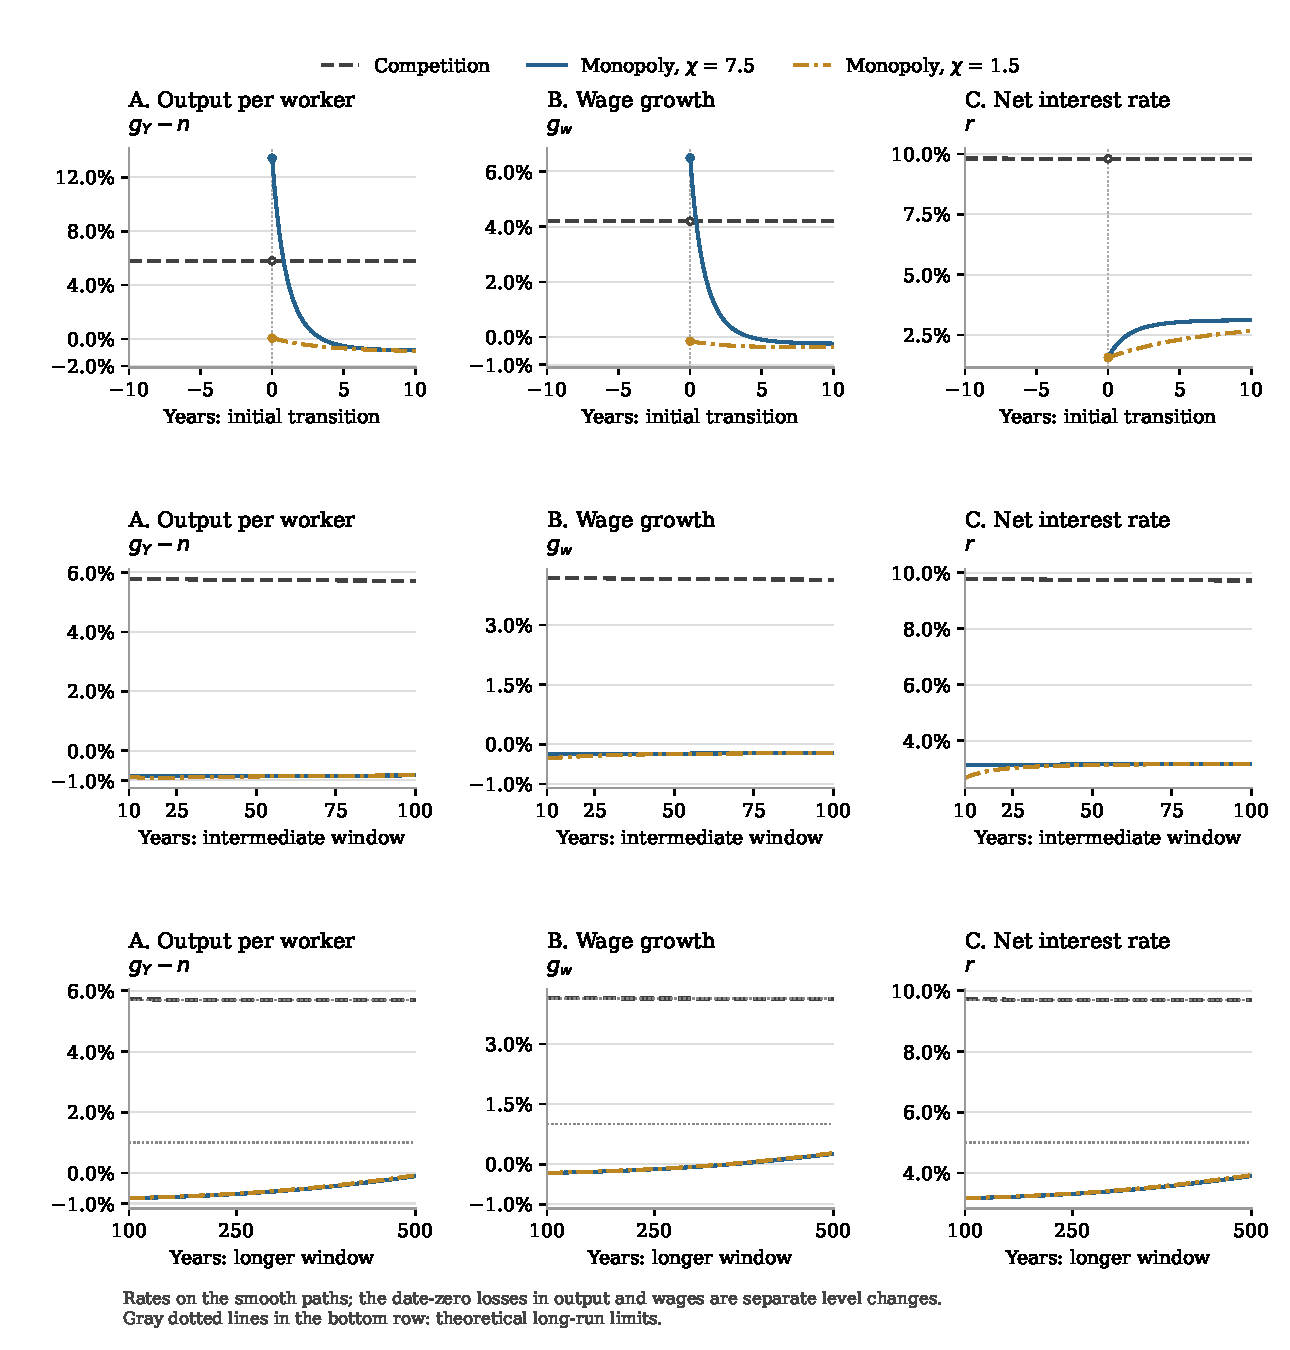
\includegraphics[width=\textwidth]{figures_rewrite/monopoly_growth_reversal_burnin/monopoly_growth_reversal_growth.pdf}
 \caption{Monopoly and the loss of AI-dominated growth: annual
 output-per-worker growth, wage growth, and net interest. Rows show
 years $-10$--10, 10--100, and 100--500. The grant occurs at zero,
 after the common competitive prehistory. Rates describe the smooth paths
 in each scenario, not the instantaneous output and wage
 losses. Gray dotted lines in the bottom row indicate theoretical
 long-run limits. Vertical scales differ across windows.}
 \label{fig:rewrite-monopoly-growth-reversal-growth}
\end{figure}

The longer windows show that the loss of sustained growth is not
confined to the initial repricing.
Under continued competition, output-per-worker growth tends to
$5.7\%$, wage growth to $4.1\%$, and the interest rate to $9.7\%$,
as in equation~\eqref{eq:rewrite-competitive-ai-growth}.
Under either monopoly path, the corresponding limits are $1.0\%$,
$1.0\%$, and $5.0\%$, consistent with the labor-bottleneck regime in
Proposition~\ref{prop:rewrite-equilibrium-regimes}. Both monopoly
economies are still adjusting at year 500: output-per-worker growth
is about $-0.1\%$, wage growth is $0.3\%$, and the interest rate is
$3.9\%$. The large stock of capital inherited from the competitive
expansion takes a long time to adjust to restricted AI supply. The
monopoly limit therefore remains distinct from the last plotted date:
monopoly removes permanently faster growth, not all long-run growth.

Figure~\ref{fig:rewrite-monopoly-growth-reversal-technology} explains
why efficiency gains do not prevent this outcome. Using the same lines
and windows, panels A--C show $B/\overline B$, AI services relative to
continued competition, and labor income as a share of output.
In the first decade, high research productivity takes efficiency to
$99.9\%$ of its upper bound, compared with $97.1\%$ under low research
productivity. Both nevertheless supply fewer AI services than continued
competition. In the longer run, efficiency approaches
$\overline B$, an improvement of $11.1\%$ over $B_0$; competition
retains $B_0$. Yet the monopoly markup prevents these improvements
from sustaining the joint expansion of capital and AI services that
occurs under competition. AI services under monopoly become negligible
\emph{relative to the competitive path}, not in absolute terms.
Labor's income share tends to $4.5\%$ under monopoly rather than zero
under competition. This larger limiting share coexists with slower
wage growth. At year 500, the labor share is still only $2.1\%$ and
$2.2\%$ under high and low research productivity, respectively,
confirming that neither path has reached its labor-bottleneck limit.

\begin{figure}[tp]
 \centering
 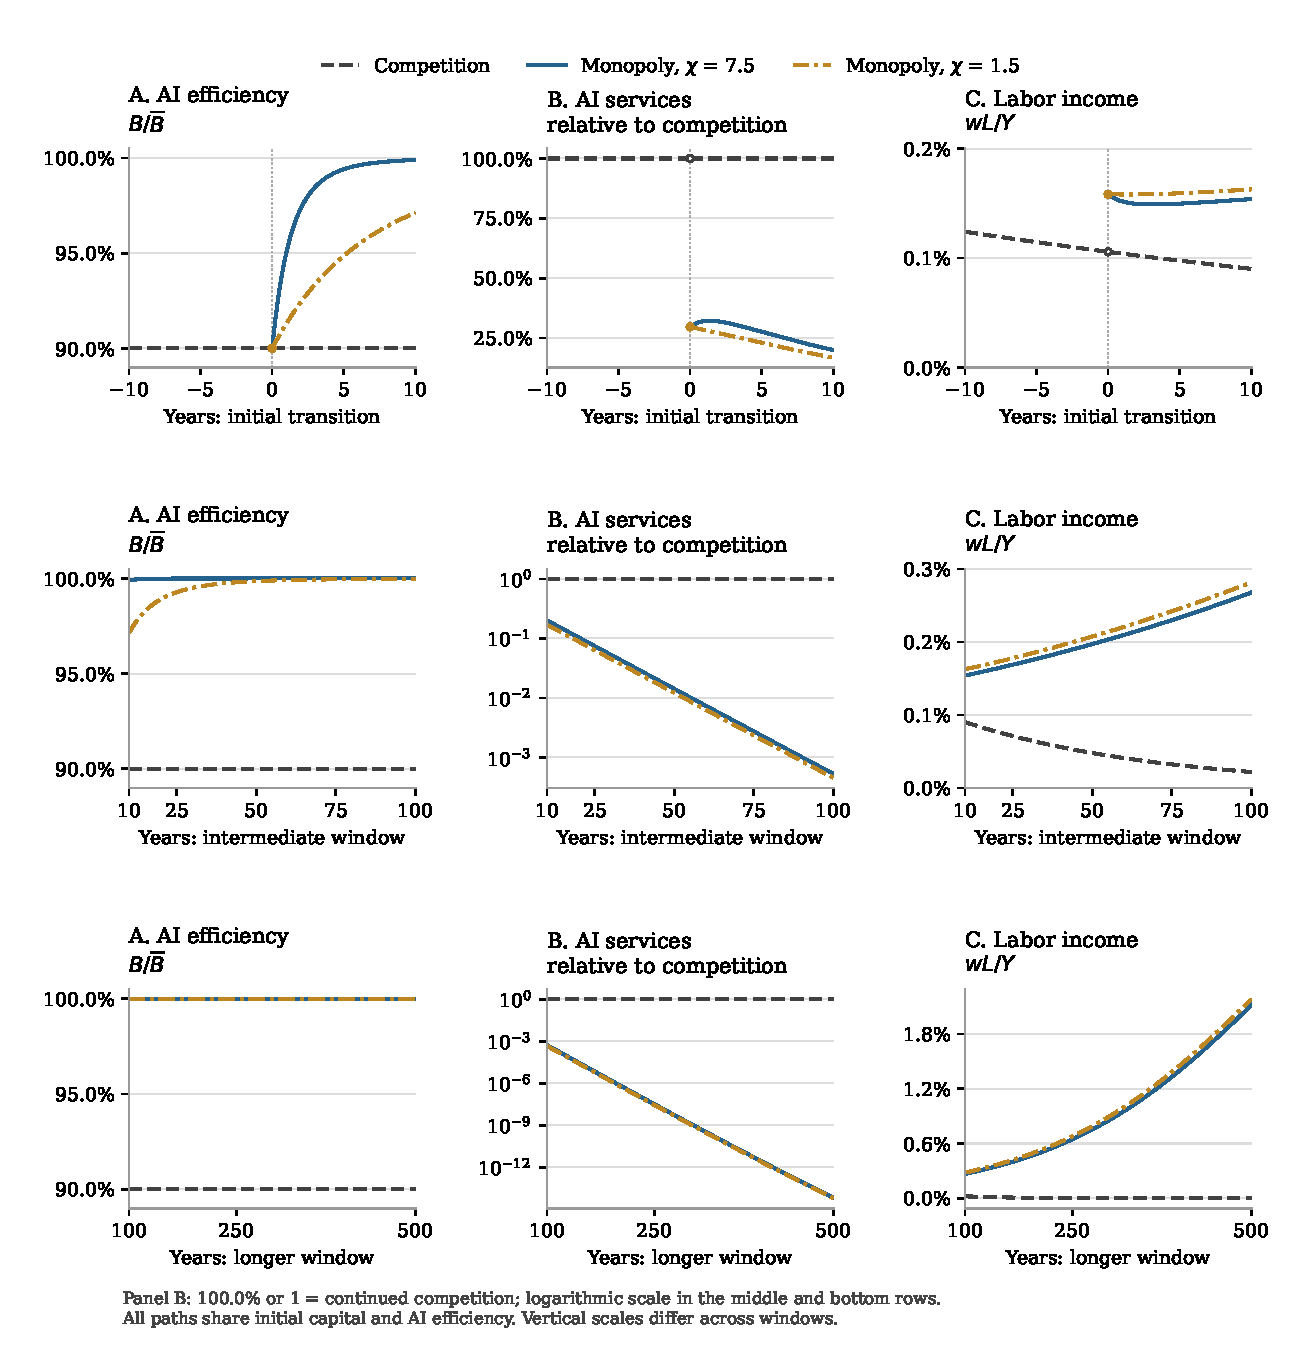
\includegraphics[width=\textwidth]{figures_rewrite/monopoly_growth_reversal_burnin/monopoly_growth_reversal_technology.pdf}
 \caption{More efficient AI but slower growth under monopoly:
 efficiency relative to its upper bound, AI services relative to
 continued competition, and labor's income share. Windows and line
 styles match Figure~\ref{fig:rewrite-monopoly-growth-reversal-growth}.
 Panel B uses percentages in the first row and multiples on logarithmic
 scales in the lower rows; its competitive benchmark is $100.0\%$ or
 one. Vertical scales differ across windows.}
 \label{fig:rewrite-monopoly-growth-reversal-technology}
\end{figure}

\Needspace{12\baselineskip}
Together with Section~\ref{subsec:rewrite-competitive-transition}, this
experiment illustrates opposite regime rankings. There,
research allows the monopoly economy with $\sigma=1.5$ to escape the
labor bottleneck from a low initial efficiency. Here, initial efficiency
already sustains AI-dominated growth under competition, and further
efficiency gains do not compensate for restricted AI use.
More efficient AI is therefore compatible with slower long-run growth.
The large initial adjustments
also reflect the abrupt withdrawal of access to existing technology.
I use it to illustrate a possible growth reversal, not to predict the
effects of an actual monopoly grant or rank household welfare.
Appendix~\ref{app:rewrite-competitive-transition} describes the additional
competitive-transition solver and numerical checks. The preceding
simulations remain separate experiments with different initial states
and efficiency bounds.
%\clearpage
